\section{Measurement Strategy}\label{s:measurement}

In this section we describe how the \inbox and \outbox coordinate to compute accurate and robust
measurements of the network conditions necessary as inputs to congestion control algorithms.

Congestion control algorithms need only a small, common set of measurements~\cite{ccp-hotnets}. 
In particular, rate-based algorithms need only three measurements: 
the sending rate, receiving rate, and path round-trip time.
A significant complication is that for accurate measurements on RTT time-scales, we must calculate send and receive rates over the same set of packets~\cite{packettrain}.
This requirement drives the design of our measurement methodology.

\subsection{Determining Epoch Boundary Packets}
\label{s:measure:marking}
Consider the stream of packets $P_B$ from all flows in a bundle $B$ in the order they leave the \inbox after scheduling.
The \inbox and \outbox need to know how to divide this stream into sets 
of packets --- which we call \emph{epochs} --- over which they can calculate measurements.
For now, we make the simplifying assumption that packets arrive at the \outbox in the same order they 
left the \inbox (we address re-ordering in Section~\ref{s:measure:limitation:reorder}). \an{note about re-ordering is a little distracting and doesn't help explain approach}
This simplifies the problem into deciding, for all given packets in $P_B$, whether it is an epoch boundary packet at which the current epoch should end and the next should begin. 
Suppose for now that we wish to have a fixed epoch size of $N$ packets.
A naive approach would be to mark the boundary between epochs every $N$ packets. 
However, this strategy is brittle; a single lost packet would de-synchronize the boxes' views of the epochs. 
More generally, any strategy that requires packet-level synchronization of the \inbox and
\outbox is untenable because any coordination would race the packets themselves.

The key idea of our methodology is that we can avoid such a synchronization problem by determining the boundary of an epoch using only information contained in the packet.
Specifically, we propose the following: a packet $p$ is an epoch boundary packet if the hash 
of some subset of its header (see below) modulo the epoch size $N$ is equal to 0, that is:
$$B(p,N) \coloneqq H(p)\ \text{mod}\ N == 0$$
Thus, an epoch boundary packet will occur (in expectation) once every $N$ packets.
For $H$, we use the Fowler/Noll/Vo (FNV) hash function~\cite{fnv-hash}, a non-cryptographic fast hash function with a low collision rate. 

\paragrapha{Choosing header subset} The header subset we use must remain constant as the packet traverses the network from the \inbox to the \outbox; otherwise, they would not be able to agree on epoch boundaries. This rules out simple approaches such as hashing the entire packet header, since the TTL field will decrement between the inbox and outbox.
Even the 5-tuple of the packet may change, since the outbox may be behind a NAT.
Using TCP sequence numbers is tempting, but retransmissions may confuse RTT measurements.

We use the IP ID field, which will change every packet. This is an imperfect solution, as modern NATs may rewrite the IP ID field~\cite{ipid}.
Ultimately, the appropriate field to use will depend on the specific deployment of \name.

\subsection{Computing Measurements}
\label{s:measure:compute}
\newcommand{\pone}{$p_{prev}$}
\newcommand{\hpone}{$h(p_{prev})$}
\newcommand{\sone}{$s_{prev}$}
\newcommand{\rone}{$r_{prev}$}
\newcommand{\ptwo}{$p_{curr}$}
\newcommand{\hptwo}{$h(p_{curr})$}
\newcommand{\stwo}{$s_{curr}$}
\newcommand{\rtwo}{$r_{curr}$}
\newcommand{\atwo}{$a_{curr}$}
\newcommand{\sentone}{$sent_{prev}$}
\newcommand{\recvdone}{$rcvd_{prev}$}
\newcommand{\senttwo}{$sent_{curr}$}
\newcommand{\recvdtwo}{$rcvd_{curr}$}


\begin{figure}
    \centering
    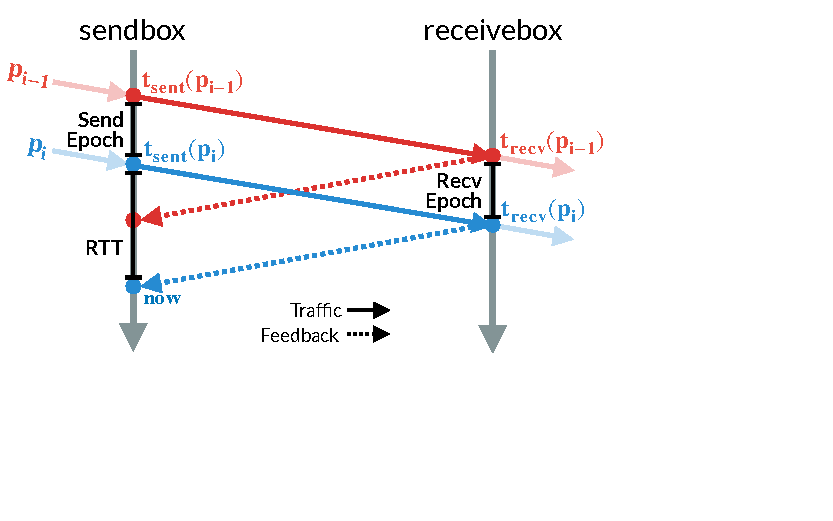
\includegraphics[width=\columnwidth]{img/rate-calculation}
    \caption{Example of epoch-based measurement calculation. Time moves from top to bottom.
    Packets from flows in a bundle
    pass through the \inbox and \outbox middleboxes on the way to their destination. When 
    the inbox observes a packet header matching the boundary condition, it records it. When
    the \outbox observes such a packet, it sends an out-of-band feedback message back to
    the \inbox, which allows it to calculate the RTT and epochs.}\label{fig:ratecalc}
\end{figure}

Given this method of marking epochs, we can now construct the procedure for computing measurements.

For a given bundle, the \inbox runs the aforementioned function on each packet $p$. Each time
the function returns true, the \inbox updates an epoch data structure that records the packet hash,
which we will call \hptwo\ for the current epoch, 
along with the current time \stwo\ and the \emph{cumulative} number of bytes sent so far, \senttwo. This structure
is sorted by the time the packet was sent, \stwo, but is indexable by the packet hash.

The \outbox runs the same function. Each time it observes a boundary packet, 
it immediately sends a feedback message to the \inbox containing the same information:
the packet hash \hptwo, the time at which it received the packet, \rtwo, and the cumulative number of bytes
\emph{received} up until that point. When the \inbox receives this feedback message at time \atwo, it looks up the
packet hash \hptwo\ in the epoch data structure, which represents the end of the current epoch,
along with the earliest boundary packet still in the data structure, \hpone\ which represents the start
of the current epoch. It now has all of the information necessary to calculate one sample of the following:
\begin{subequations}
    \begin{align}
        RTT &= &now - s_2 \\
        send\_epoch\_duration &= &s_2 - s_1\\
        recv\_epoch\_duration &= &r_2 - r_1\\
        bytes\_sent\_in\_epoch &= &bytes\_sent\ at\ s_2 &\ - \\
                                    &&bytes\_sent\ at\ s_1&\notag\\
        bytes\_rcvd\_in\_epoch &= &bytes\_rcvd\ at\ r_2 &\ - \\
                                &&bytes\_rcvd\ at\ r_1\notag\\
        send\_rate &= &\frac{bytes\_sent\_in\_epoch}{send\_epoch\_duration}\\
        recv\_rate &= &\frac{bytes\_rcvd\_in\_epoch}{recv\_epoch\_duration}
    \end{align}
\end{subequations}
%(Note $bytes\_rcvd\_in\_epoch$ can also be interpreted as the number of bytes
%acknowledged for that epoch, which is a common signal used by many conestion
%control algorithms.)
Finally, it clears all marked packets preceeding \ptwo\ leaving \ptwo\
to be the start of the next epoch.


\subsection{What About Lost Packets?}
\label{s:measure:loss}
This method is robust to the loss of boundary packets between the \inbox and \outbox.
Suppose the \inbox sees boundary packets $p_1, p_2, p_3$, but $p_2$ is lost after passing through
the \inbox so the \inbox only receives feedback for $p_1$ and $p_3$. Upon receiving $p_1$, 
the \inbox will truncate its data structure up until $p_1$. Upon receiving $p_3$, the \inbox 
looks up the oldest remaining boundary packet, $p_1$, and considers that the beginning of the epoch.
As a result, the epoch is longer than intended, but no measurements are lost or corrupted. 
The same argument applies to the loss of feedback messages. 
The key here is that the \inbox actually calculates both the send and receive epoch based on information
from the \outbox rather than the \outbox deciding what consitutes an epoch on its own. 

\subsection{Fault Tolerance}\label{s:impl:ft}
\an{perhaps redundant, moved from \S\ref{s:impl}}
\begin{outline}
\1 If outbox feedback is lost, the next outbox feedback that is successfully received at the inbox will determine the end of the measurement epoch.
    \2 The measurements will still be accurate, but they will end up being taken over a longer period than intended.
\1 The inbox dynamically sets the epoch duration to be (rate * rtt) rounded down to the nearest power of two. It then communicates the epoch duration to the outbox.
    \2 If this communication is lost, since the epoch duration is set to be a power of two, the inbox and outbox will still agree on a set of epoch packets.
\1 If the inbox crashes, the operator can remove it from the service chain, and performance will be no worse than it is today.
\1 If the outbox crashes, after a timeout period, the inbox will disable aggregation on the path and performance will be no worse than it is today.
\end{outline}


\subsection{Choosing The Epoch Size}
\label{s:measure:epoch}
How do we choose the number of packets that should be in each epoch?
In 3.1, we assumed a fixed epoch size of $N$ packets.
However, in practice, the epoch must be a function of the sending rate.
If the epoch size is too small relative to the rate,
the epochs will be easily influenced by bursts and thus the measurements will be highly variable
and not useful.
If the epoch size is too large relative to the rate, the congestion control algorithm will not
receive feedback frequently enough to respond promptly to changing network conditions. 
As shown in prior work, congestion control algorithms can behave properly even if their
signals are only updated roughly once per RTT~\cite{ccp-hotnets}.
Setting the epoch size equal to our estimate of the number of packets currently inflight 
(our current sending rate multipled by our current esimate of the RTT) will yield roughly
one epoch and thus a new set of measurements per RTT.

Since the rate and thus the number of inflight packets is continuously changing over time,
we need to continually update the epoch size. Rather than using exactly the number of inflight
bytes, we round the value down to the nearest power of two so that the new epoch size is
always a multiple of the old one and thus will be compatible. 

For examaple, \fc{is an example necessary?}
if the inbox is marking every 256 packets
and the \outbox is marking every 512 packets, 
the inbox is just marking a super set of the \outbox packets, 
so it is effectively equivalent to them both marking every 512 packets.
    
\subsection{Microbenchmarks}
\label{s:measure:microbench}
    \fc{Maybe this fits better in eval}

    How well do our estimates match the actual signals? In Figure X, we sample a two minute segment from 
    one experiment in our evaluation section and plot the \inbox's estimated values 
    of the RTT and receieve rate compared to the actual RTT and the rate of packets leaving 
    the bottleneck router over time. We find, \fc{...}. The absolute difference between the values
    across time is 

    More generally, we compute the total absolute difference beween the estimated and actual values over the
    course of all experiments in our evaluation, and plot the distributution in Figure Y.
    
\subsection{Limitations}
\subsubsection{Re-Ordering}
\label{s:measure:limitation:reorder}
Earlier we ignored re-ordering of packets between the \inbox and \outbox. However, if packets
are re-ordered, the \inbox and \outbox will observe a different view of the same epoch.
For example, consider packets numbered 1 to 20, where 10 is a boundary packet. The \inbox observes
10 packets in each epoch: [1,10] in epoch 1 and [11,20] in epoch 2. 
However, suppose packet 7 is delayed and arrives after packet 10. The \outbox will observe 9
packets in epoch 1 and 11 packets in epoch 2. 
Spurious re-ordering can be compensated by using an EWMA across epochs rather than the raw values
calculated at each epoch. If there is persitent re-ordering, it may be necessary to add a constant 
value to either the send or receive rate to compensate.

\subsubsection{Suitable Algorithms}
\label{s:measure:limitation:algs}
The set of measurements we obtain are sufficient for most rate-based algorithms, but may not be 
suitable for traditional window-based algorithms which require low-level metrics such as 
the number of inflight packets or number of packets lost. Although it should be possible
to compute these from the measurements we already collect in an ideal scenario, they would easily
break in the presence of network anomilies such as re-ordering. Thus, we leave the development
of robust signals for window-based algorithms to fuure work. 
Thus, \name currently operates best with rate-based algorithms such as BBR, Nimbus, or Copa~\cite{bbr,nimbus,copa}.
